\subsection{Kanter}\label{subsec:kant}
Som nævnt er kanter ikke lokalt distinkte. Kanter kan dog bruges til at fjerne en del unødvendig information fra et billedet, ved kun at udtrykke kanterne.  En kant kan defineres ved at opfatte billedet som en funktion $f$, der afbilder billedintensiteten i 1-dimension. En høj kurve, angiver et skarpt intensitetsskift og derved en kant som i figur \ref{fig:kant}.
\noindent
\begin{figure}[H]
    \centering
    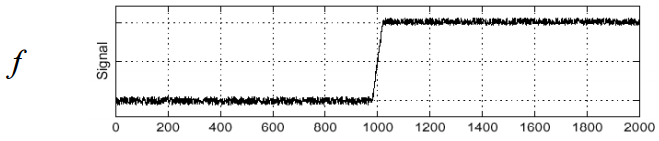
\includegraphics[width=0.55\textwidth]{fig/7.png}
     \vspace{-1em}
    \begin{center}        
     \caption{\textcolor{gray}{\footnotesize \textit{
     En 1-dimensional fortolkning af intensiteten i et billede. De små udsving indikere støj, den store kurve repræsenter et skrapt skift i intensiteten og derved en kant i et billedet.}}}
    \label{fig:kant}
     \end{center}
       \vspace{-2.5em}
  \end{figure}
\noindent
En differentiering af funktionen fra figur \ref{fig:kant} vil angive, hvor skarp kurven er og derved fremhæve dens udsving. Et 2-dimensionelt billede er ikke en kontinuerlig funktion, men består af diskrete værdier i form af pixel informationer.
Billedet differentieres derfor ved en approksimeret differentiering: \begin{equation}
\dfrac{df(x)}{dx}=\dfrac{f(x+1)-f(x-1)}{2}
\label{diff}
\end{equation}
\eqref{diff} kan udføres på billedet ved at folde billedet med kernen $[1 \hspace{0.5cm} 0 \hspace{0.5cm} -1]$. Foldning af et billede \emph{I} med indgangen $(M \times N)$, med en kerne \emph{K} med indgangen $(m \times n)$ , defineres ved operatoren: $I\ast K$ og udføres ved, for hvert punkt i billedet ved at udregne:
\begin{equation}
O(i,j) = \sum\limits_{k=1}^m \sum\limits_{l=1}^m I(i+k-1,l-1)K(k,l)
\end{equation}
Problemet ved differentiering, visualiseret i figur \ref{fig:kant}, er at støj i billedet (de små udsving) også vil blive fremhævet, hvilket kan resultere i fejlagtige detektioner af kanter. For at fjerne støjen foldes billedet med et Gaussisk filter, hvilket er en diskret approksimering til den Gaussiske funktion. Det Gaussiske filter beskriver et punkt, ved en vægtet normalfordeling af de omkringliggende pixelværdier. Foldning af et billede med et Gaussisk filter vil resultere i en "flydende" overgang mellem pixel værdierne og derfor glatte billedet.  Den Gaussiske funktion i 2-D, hvor $ \sigma $ er standardafvigelsen af den Gaussiske fordelingen, er defineret som:
\begin{equation}
G(x,y,\sigma) = \frac{1}{2 \pi \sigma ^{2}} e^{- \frac{x^{2} + y^{2}}{2 \sigma ^{2}}}
\label{2dgaussian}
\end{equation} 
For at undgå itereration af billedet to gange, for differentiering og sløring, kan dette udføres i en samlet operation, ved at folde billedet med et differentieret Gaussisk filter, da foldning er en associativ operation.
\begin{equation}
\dfrac{\partial}{\partial x}(G \ast f) = (\dfrac{\partial}{\partial x}G) \ast f
\end{equation}
Udføres ovenstående på signalet fra figur \ref{fig:kant} vil det resultere i et "bakke" formet signal, hvor bakken indikere en kant. For en mere lokaliserbar kant, kan den dobbelt afledte tages, som set i figur \ref{fig:deriv}.
\begin{figure}[H]
    \centering
    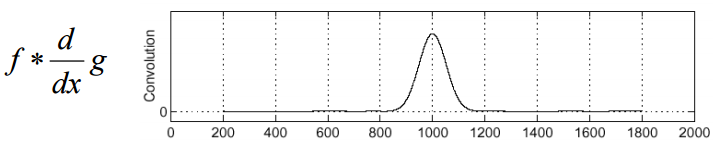
\includegraphics[width=0.55\textwidth]{fig/8.png}
    \vspace{-1em}   
    \begin{center}
    \caption{\textcolor{gray}{\footnotesize \textit{
     Resultatet af at folde et dobbelt differentieret Gaussisk filter med funktionen}}}
    \label{fig:deriv}
     \end{center}
    \vspace{-2.5em}  
  \end{figure}
\noindent
Kanten er nu let definerbar, ved at lokalisere når funktionen krydser nul. <I et 2-dimensionelt billede repræsentere intensitetsskift også en orientering. Vertikale kanter findes ved at folde billedet med et Gaussisk filter, differentieret i x-aksen og y-aksen for horisontale kanter.>